\chapter{Results exploitation}

\begin{summary}
\lipsum[1]
\end{summary}

\section{Introduction}
In Chapter \ref{cha:model} we have shown how a 3D-SIC can be modelled and the problem we are dealing with in this work, as well as simulation results based on multi-objective optimization. In Chapter \ref{cha:robustness}, we have shown that the methodology can show good convergence and diversity properties even if the problem contains criteria of heterogeneous nature. In this Chapter, we will discuss about how a designer could use these results and take advantage of a multi-criteria oriented methodology in the process of producing a 3D-SIC to, for instance, make a choice among the solutions of the Pareto frontier.

\section{Preference modelling}
As explained in Chapter \ref{cha:rol.mcda}, once a Pareto front has been determined or approximated, the next step is to choose among this set of solutions. One way to help decision makers to make their choice is to model their preferences, for instance with an outranking method. In the scope of this work, we will present the use of the PROMETHEE methodology as it has been developed in our department and has also shown good results in different fields \cite{Beh2010}.

\subsection{PROMETHEE model}
In order to use the PROMETHEE method, the decision maker has to inform about his preferences on the criteria, these being preference functions, indifference and preference thresholds and weights on the criteria (see Chapter \ref{cha:rol.mcda}). To illustrate this, we will use a PROMETHEE software called D-Sight that has been developed by Quantin Hayez and use the results of the simulations presented in Chapter \ref{cha:robustness}.

\begin{figure}[h!]
\begin{center}
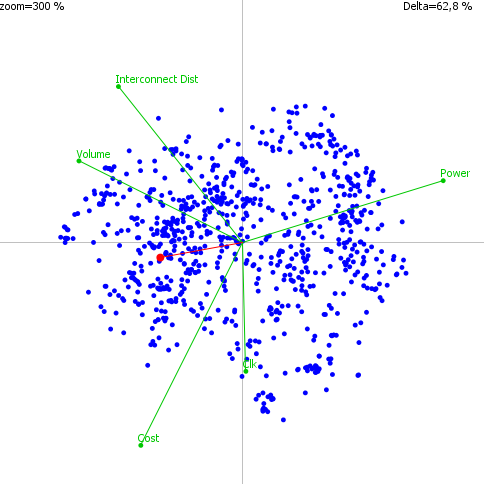
\includegraphics[width=0.8\linewidth]{gva804}
\end{center}
\caption{GAIA plane of the case study}
\label{fig:gva804}
\end{figure}

\begin{figure}[h!]
\begin{center}
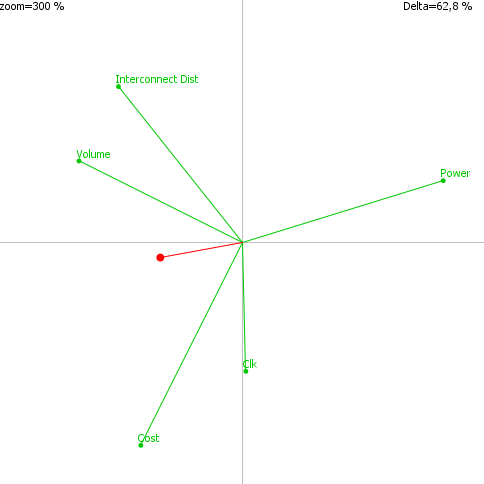
\includegraphics[width=0.8\linewidth]{gva804crit}
\end{center}
\caption{GAIA plane of the case study (criteria axis only)}
\label{fig:gva804crit}
\end{figure}

\section{How to pertinently represent multi-criteria information}


\section{On the use of a multi-criteria paradigm in microelectronics design}
As described in Chapter \ref{cha:rol.icdesign}, the multi-criteria paradigm is rarely used in the field of IC design; at best, trade-off analyses are performed. To our knowledge, more global multi-criteria analyses have not been carried out yet.

When discussing with design experts, it is quite interesting to see how they easily understand the stake of the MCDA paradigm and how it would be able to help designers facing IC development challenges. However, it is more difficult to make them adopt this approach for three main reasons that have appeared throughout several discussions:

\begin{enumerate}
\item "It is not how we optimise circuits" seems to be one of the most frequent statements. Indeed, the industry follows a uni-criterion paradigm and is not used to first explore several possible solutions and then determine good compromise solutions. The designers will generally decide about an architecture and try to optimise it to achieve the specifications.
\item Designers can understand how preference modelling work, however they are not used to answer questions about indifference/preference thresholds or criteria weights as they receive specifications to achieve. This would need a change in how the design of a circuit is approached and how specifications are formulated.
\item As a consequence of the fact that design space exploration is based on performance assessment, preference modelling would be based on estimated metrics. While it will provide relevant ordered information, this will not necessarily match the values of real specifications. Therefore, this adds a level of difficulty for the modelling.
\end{enumerate}



\section{Conclusion}